\section{Network Flow}
	\hspace{10mm}This section will show through description and screenshots how the fabsec-network will come to life, as well as how it is used to commit log entries to the blockchain, and how the frontend allows a user to see those log entries for themselves.\\
	
	\hspace{10mm}First, let's start with a listing of scripts as mentioned above. You can see their numbering (or lettering for the meta-scripts) and names:
	
		\begin{figure}[H]
		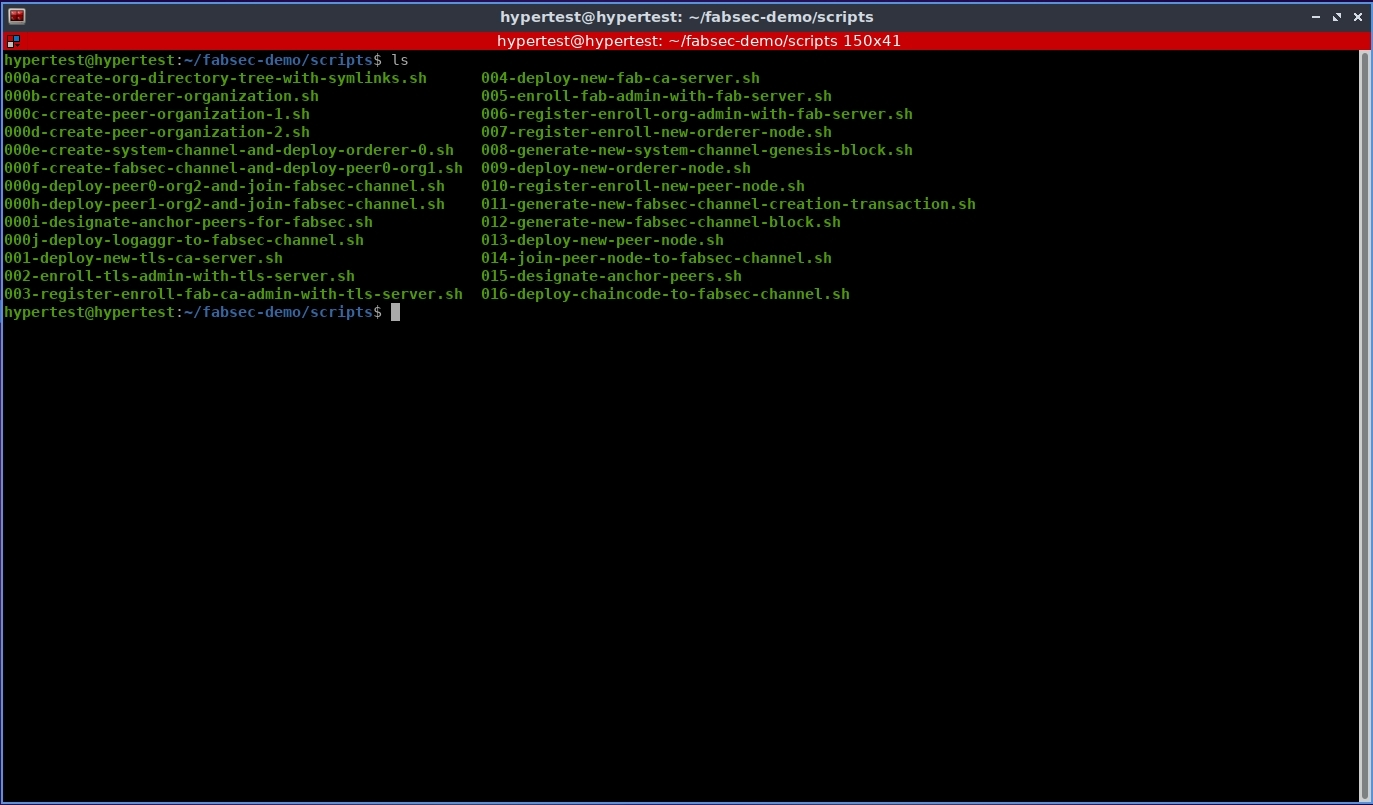
\includegraphics[width=\textwidth]{./fabsec-report-network-flow/network-flow-1.jpg}
		\caption{A Directory Listing of scripts/}
		\end{figure}
	
	\newpage	
	\hspace{10mm}Next, we create the Organization Directory Tree with script 000a:
	
		\begin{figure}[H]
		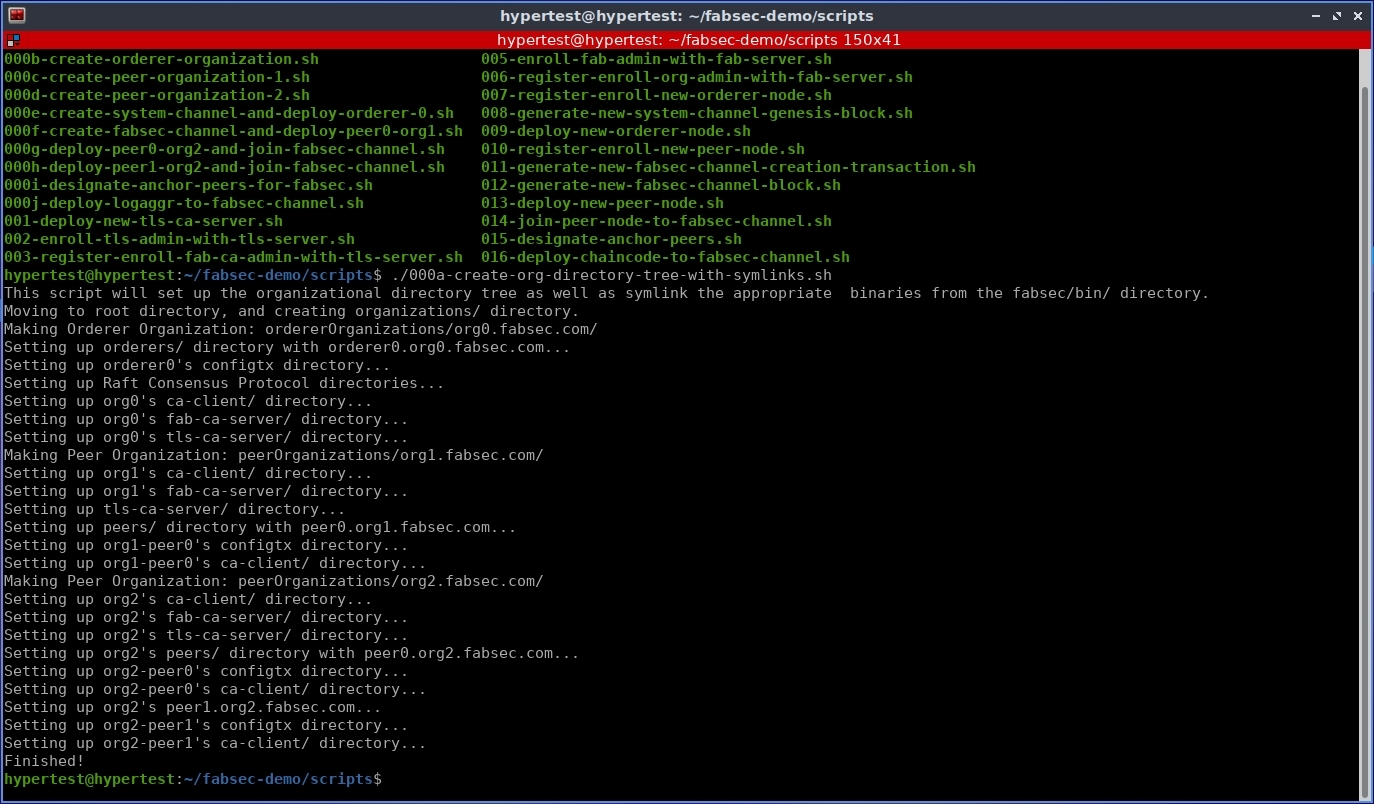
\includegraphics[width=\textwidth]{./fabsec-report-network-flow/network-flow-2.jpg}
		\caption{The Creation of the Base Organization Tree}
		\end{figure}
	
	\newpage
	\hspace{10mm}Then, we register and enroll the Administrators. One for the TLS CA Server, one for the Fabric CA Server, and the Organizational Admin. This is done through the scripts 000b, 000c, and 000d. Since it's similar output for all of them, here are two screenshots of 000b in action:
	
		\begin{figure}[H]
		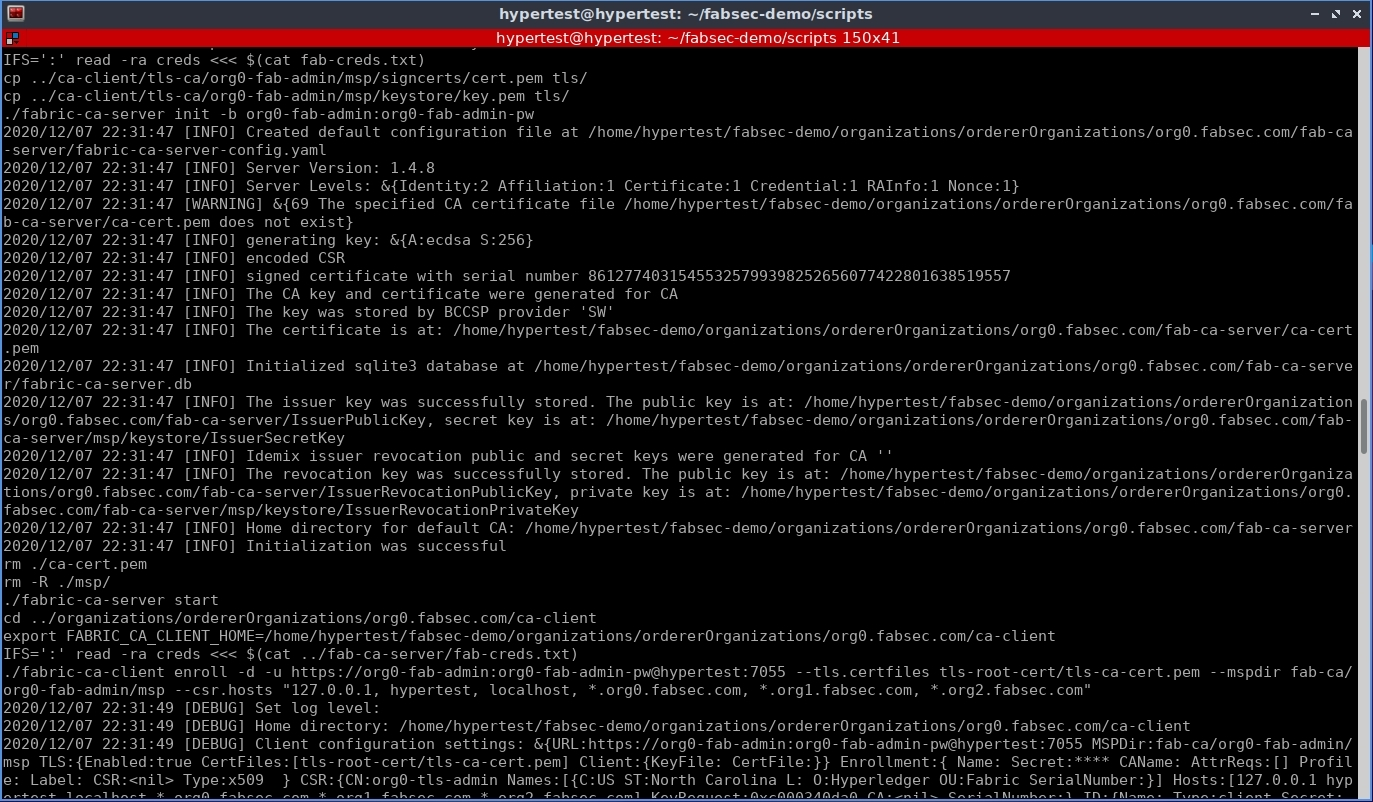
\includegraphics[width=.8\textwidth]{./fabsec-report-network-flow/network-flow-3.jpg}
		\centering
		\caption{Middle Output of the Organization0 Creation Script}
		\end{figure}
		
		\begin{figure}[H]
		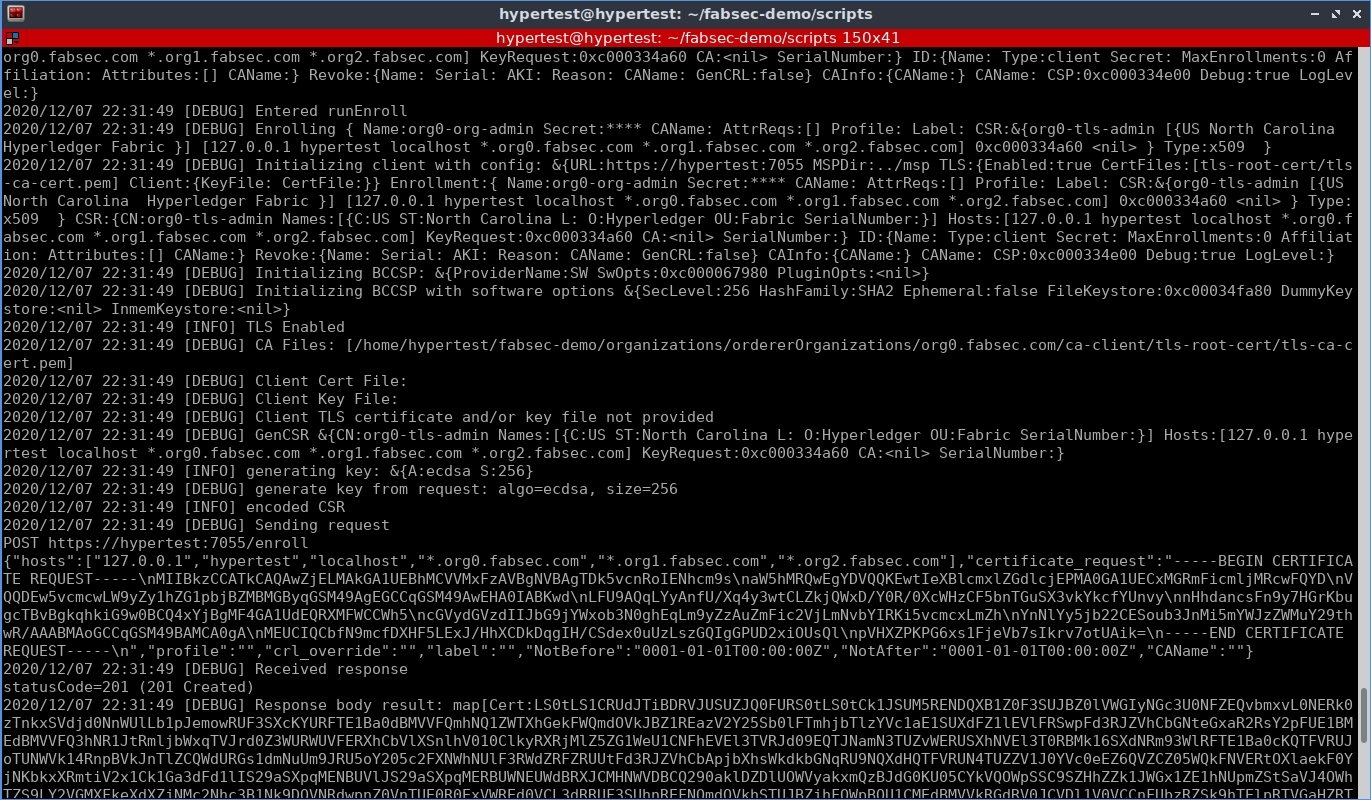
\includegraphics[width=.8\textwidth]{./fabsec-report-network-flow/network-flow-4.jpg}
		\centering
		\caption{End Output of the Organization0 Creation Script}
		\end{figure}
		
	\newpage
	\hspace{10mm}In the next phase, we start up the Orderer. Here you can see the orderer's output: how it starts the system-channel and start doing its Raft initialization:
	
		\begin{figure}[H]
		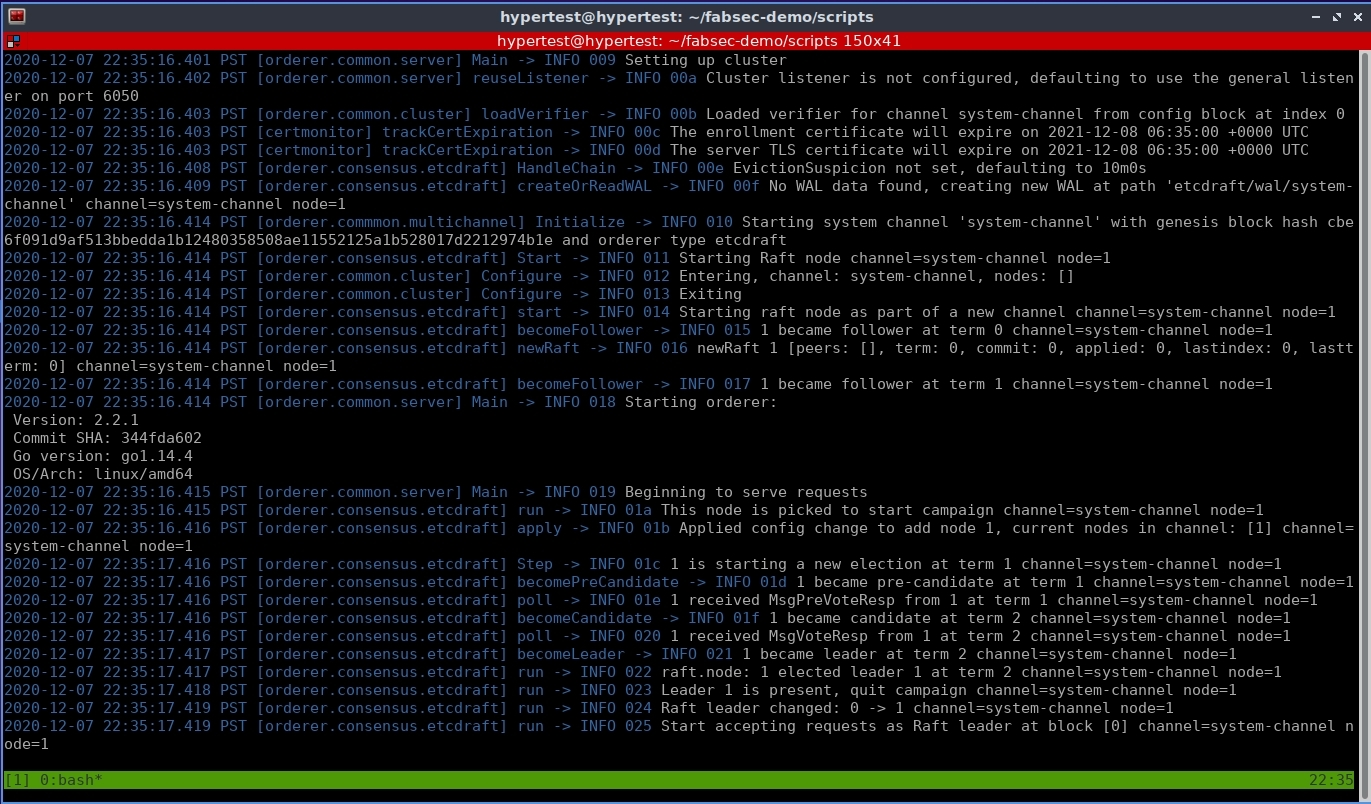
\includegraphics[width=\textwidth]{./fabsec-report-network-flow/network-flow-5.jpg}
		\caption{orderer0 Output including Raft Details}
		\end{figure}
		
	\newpage
	\hspace{10mm}The next two screenshots show peer0 booting up. The first one is just a view of peer0 starting up, and the second is the end of peer0's boot cycle, and how orderer0 has reacted to it:
	
		\begin{figure}[H]
		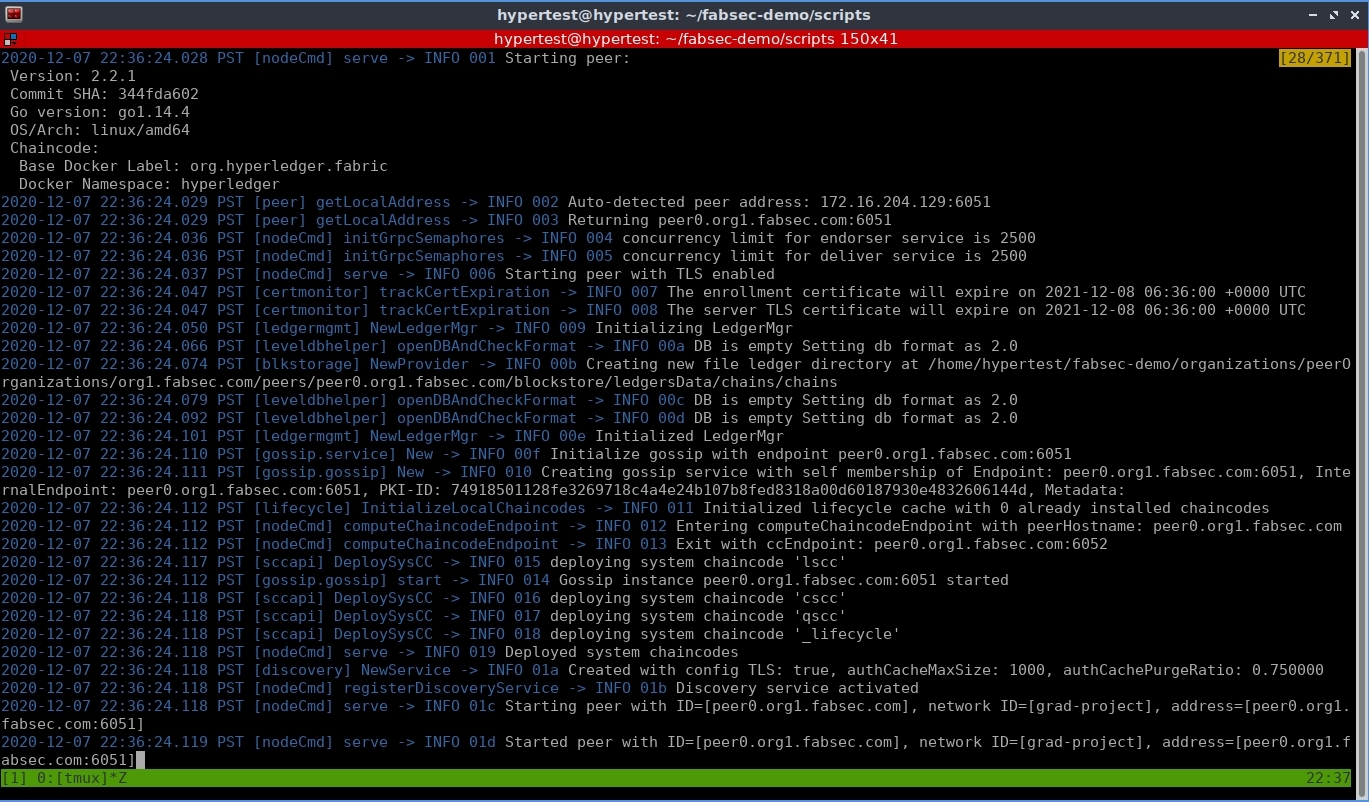
\includegraphics[width=.8\textwidth]{./fabsec-report-network-flow/network-flow-6.jpg}
		\centering
		\caption{peer0 Initial Boot}
		\end{figure}
		
		\begin{figure}[H]
		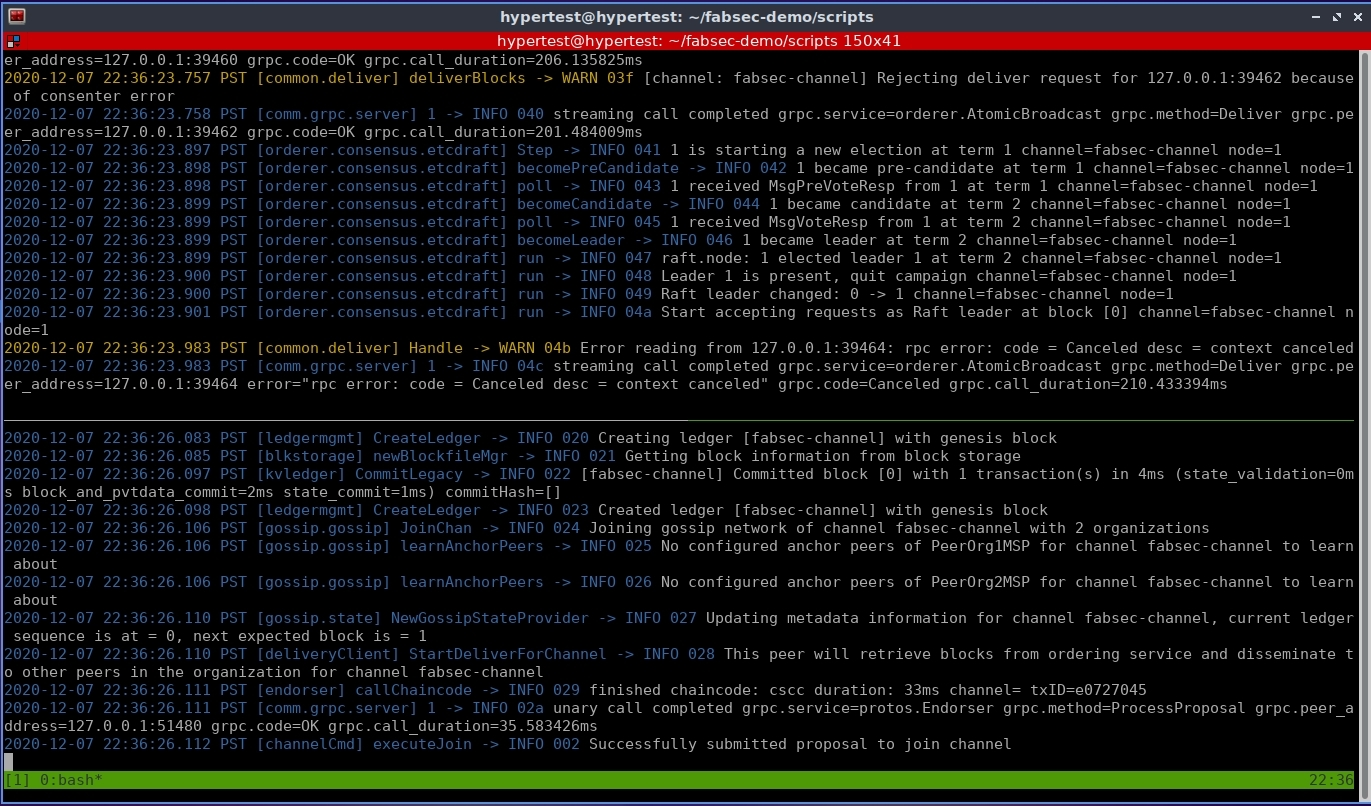
\includegraphics[width=.8\textwidth]{./fabsec-report-network-flow/network-flow-7.jpg}
		\centering
		\caption{peer0 End of Boot and orderer0 Reaction}
		\end{figure}
		
	\newpage
	\hspace{10mm}Since the start-up output of the other Peers is pretty similar, here is a \textit{tmux}'d sceenshot over the Orderer and the three Peers. orderer0.org0 is in the top left, peer0.org1 is in the bottom left, peer0.org2 is in the top right, and peer1.org2 is in the bottom right. Notice out peers 0 and 1 of Org2 can already see each other. This is because intra-organization gossip is already going. For inter-organizational gossip, we have to run the Designate Anchor Peer script:
	
		\begin{figure}[H]
		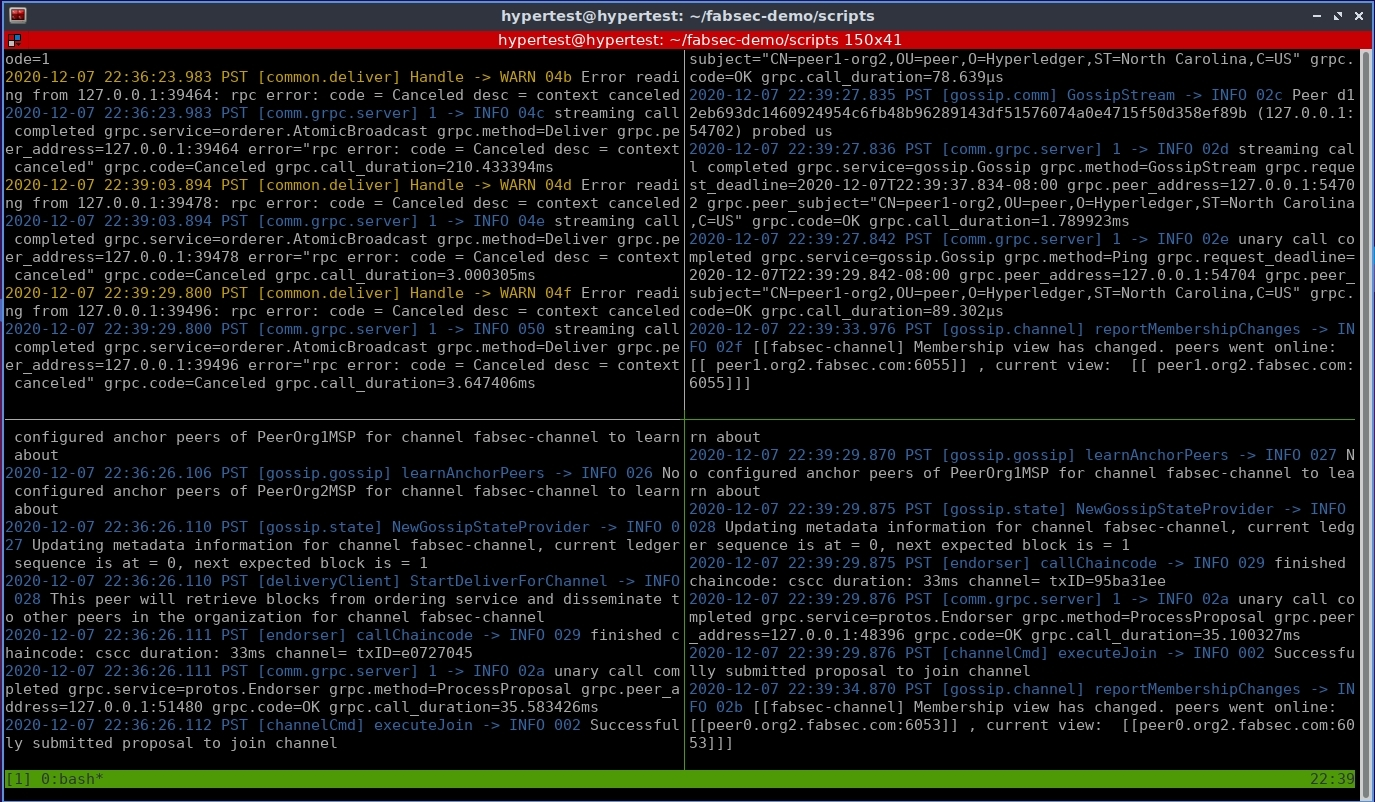
\includegraphics[width=\textwidth]{./fabsec-report-network-flow/network-flow-8.jpg}
		\caption{\textit{tmux}'d view of the Orderer and All Three Peers}
		\end{figure}
		
	\newpage
	\hspace{10mm}These next three screenshots are after script 000i, the Designate Anchor Peers script is ran. The first two show the output of the fetching, modifying, and resubmitting of the Configuration Block (also known as the Genesis Block) from/to the Orderer for peer0.org1. (Even though I don't show it the same thing happens with peer0.org2.) The third screenshot shows how the peers react to this new configuation block coming it. As you'll see peer0.org1 (bottom left) and peer0.org2 (top right) now see each other and updated their network view accordingly, however peer1.org2 (bottom right) is strictly an internal node, and therefore won't update their view.
	
		\begin{figure}[H]
		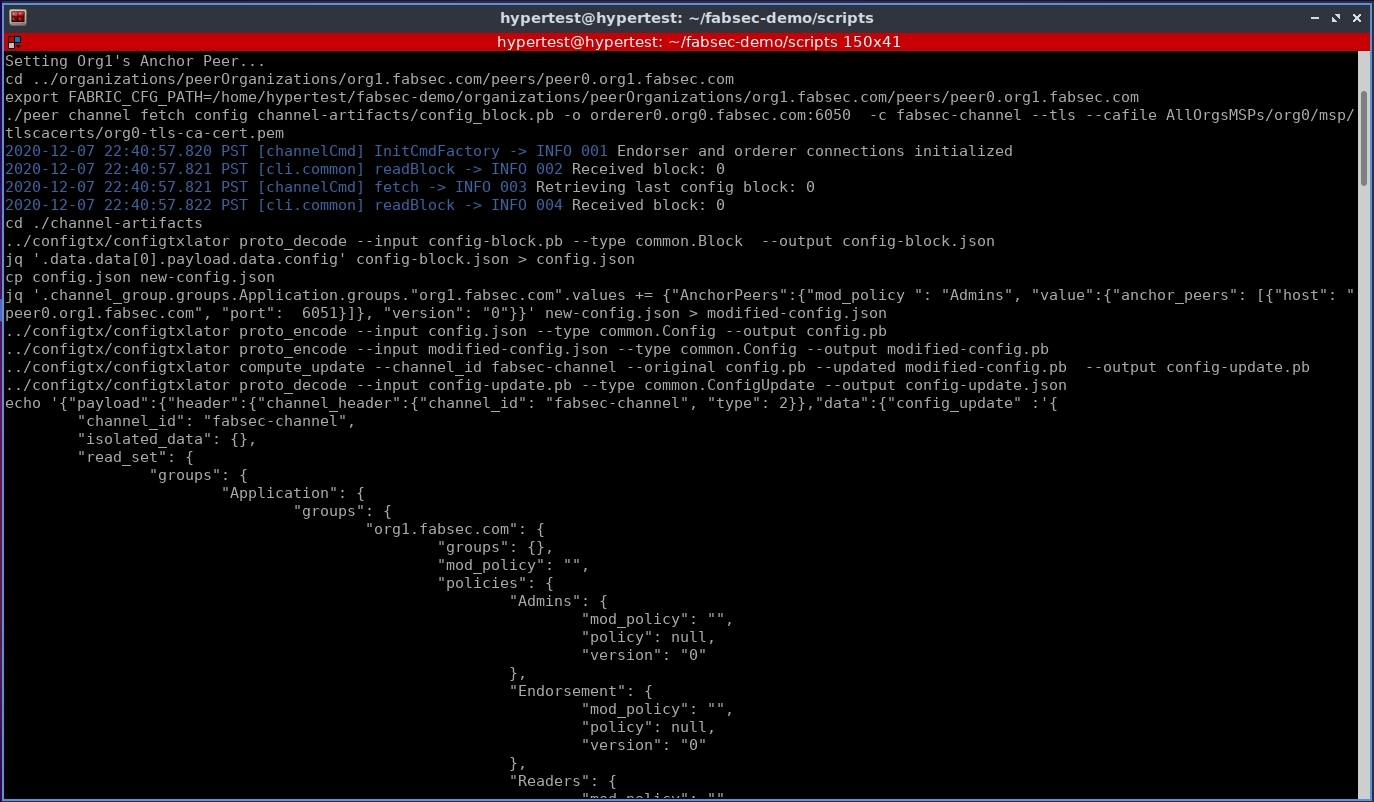
\includegraphics[width=\textwidth]{./fabsec-report-network-flow/network-flow-9.jpg}
		\caption{Beginning of 000i Script's Output peer0.org1}
		\end{figure}
		
		\begin{figure}[H]
		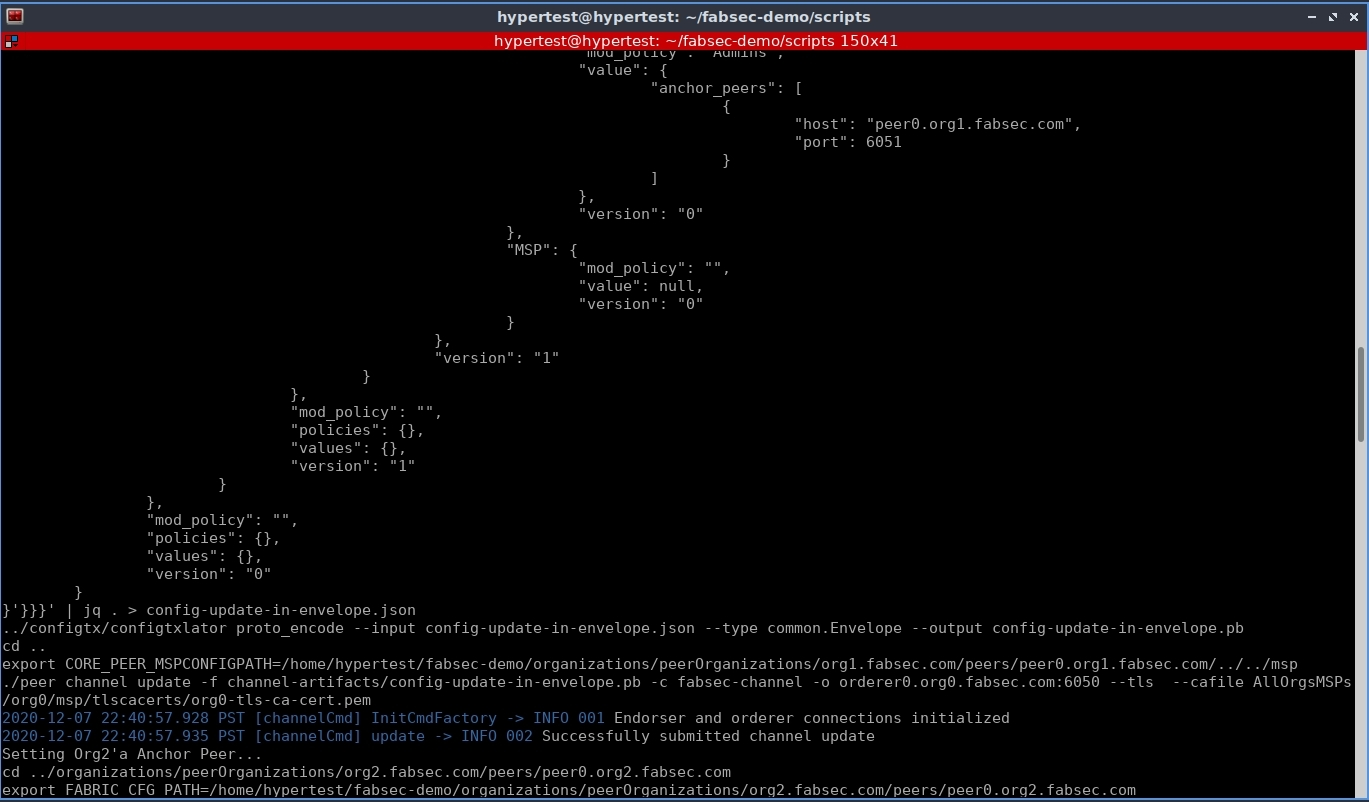
\includegraphics[width=.9\textwidth]{./fabsec-report-network-flow/network-flow-10.jpg}
		\centering
		\caption{End of 000i Script's Output for peer0.org1}
		\end{figure}
		
		\begin{figure}[H]
		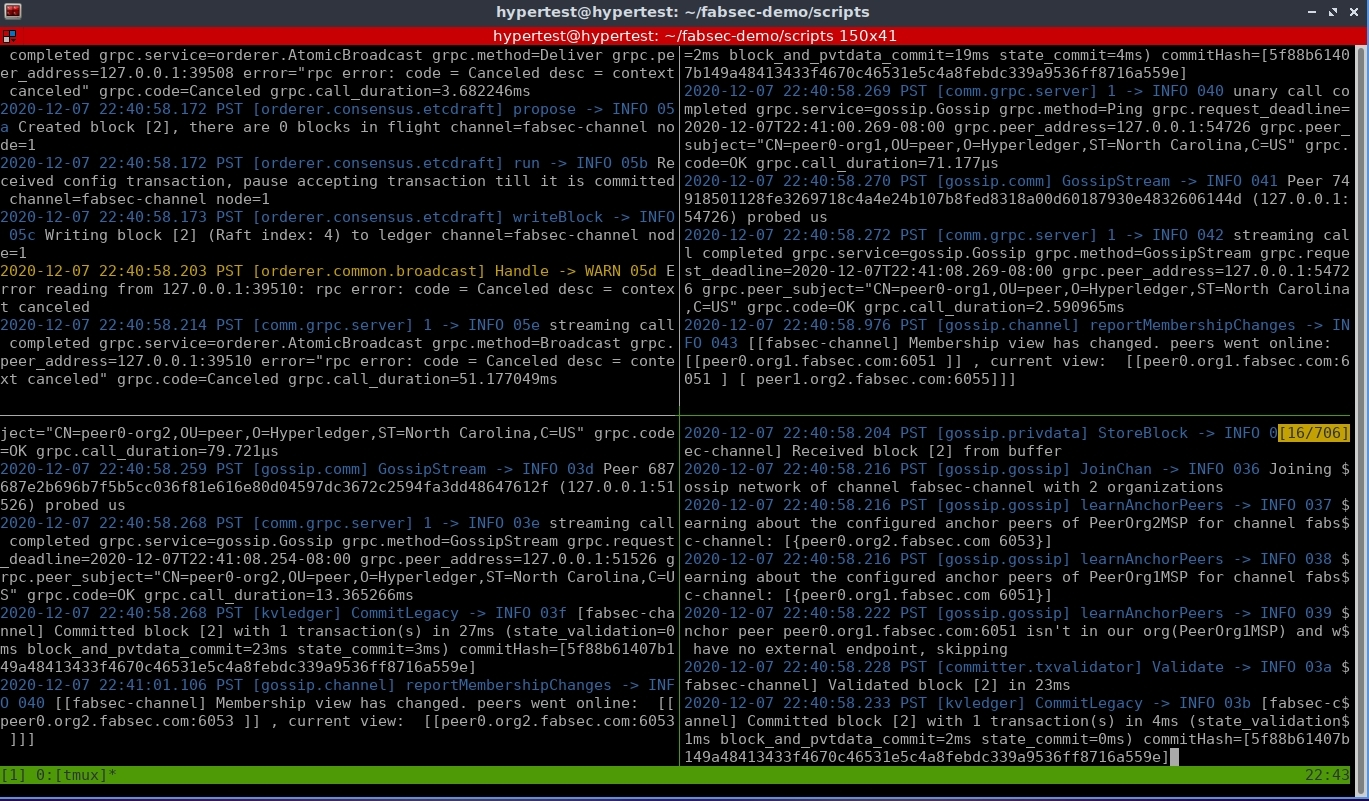
\includegraphics[width=.9\textwidth]{./fabsec-report-network-flow/network-flow-11.jpg}
		\centering
		\caption{Updated Peer Network View After Modified Config}
		\end{figure}		
		
	\newpage
	\hspace{10mm}Now that the network is essentially fully realized from a topography point-of-view. We can deploy the Chaincode to the peers. The first screenshot will show the packaging, installing, and approval of the chaincode. The second will show the committing and they values returned by the peers. As mentioned before, the Chaincode runs in its own Docker container on the Peer, so the second screenshot also shows those Docker containers running the Chaincode. Notice how there are three containers running; one for each peer. Finally the third screenshot will show the view of the peers just after they have committed the chaincode.
	
		\begin{figure}[H]
		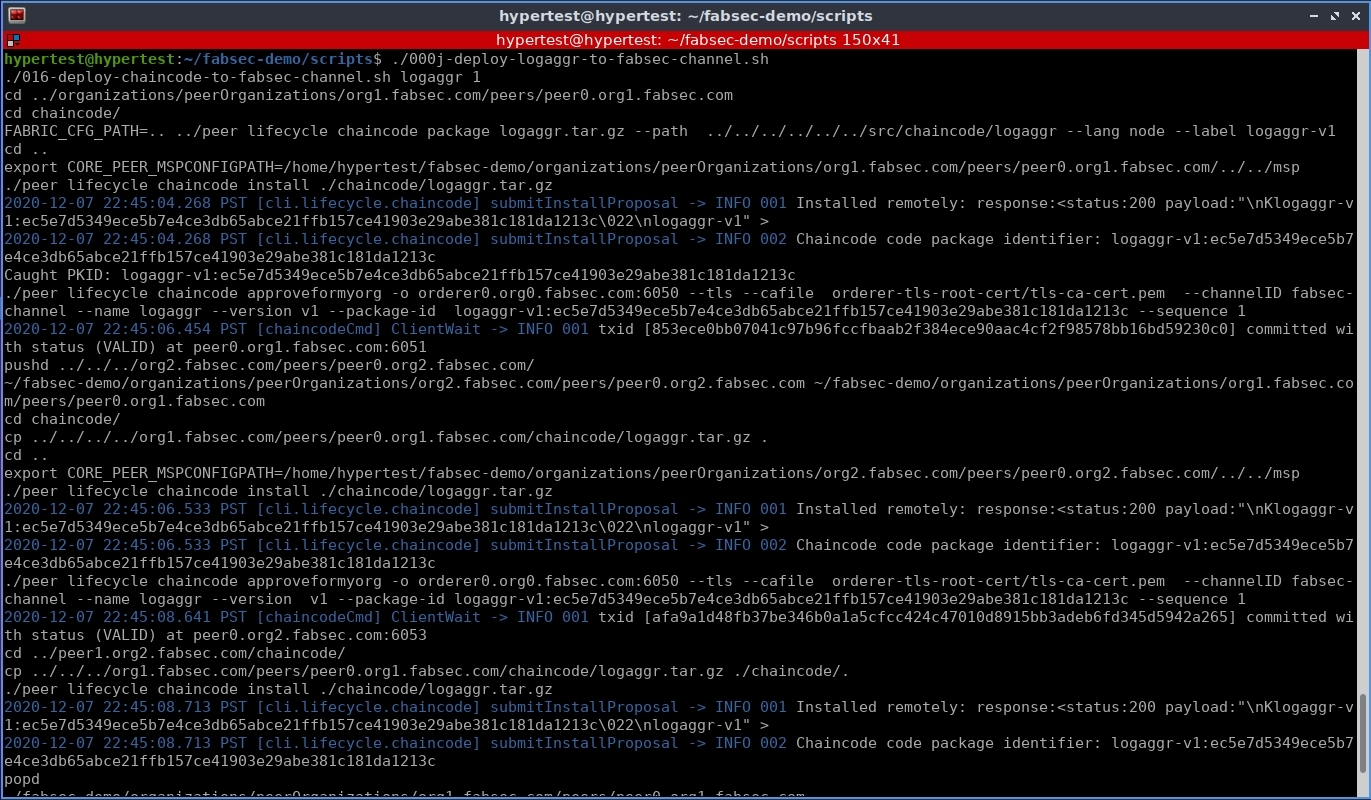
\includegraphics[width=\textwidth]{./fabsec-report-network-flow/network-flow-12.jpg}
		\caption{Packaging, Install, and Approving the Chaincode}
		\end{figure}
		
		\begin{figure}[H]
		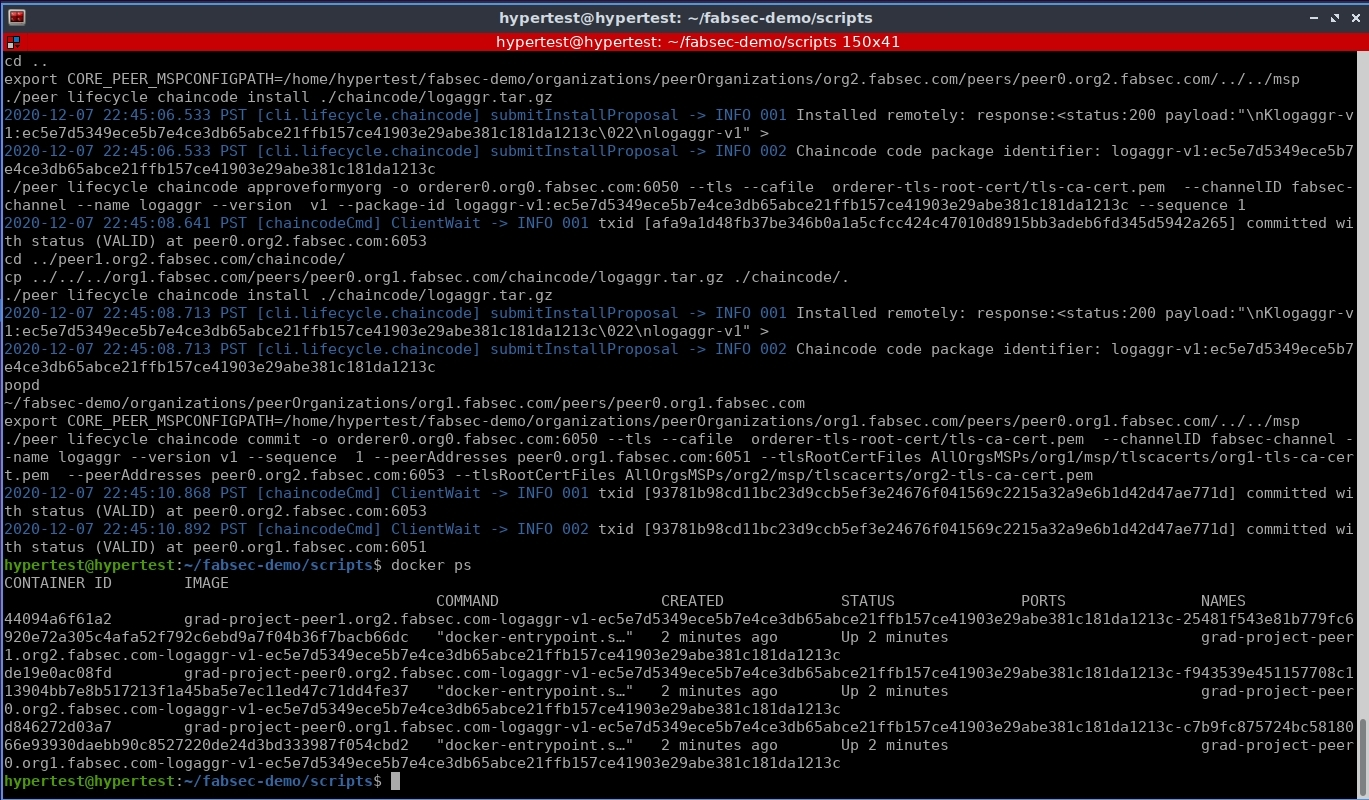
\includegraphics[width=.9\textwidth]{./fabsec-report-network-flow/network-flow-13.jpg}
		\centering
		\caption{Committing the Chaincode and \textit{docker ps} View}
		\end{figure}
		
		\begin{figure}[H]
		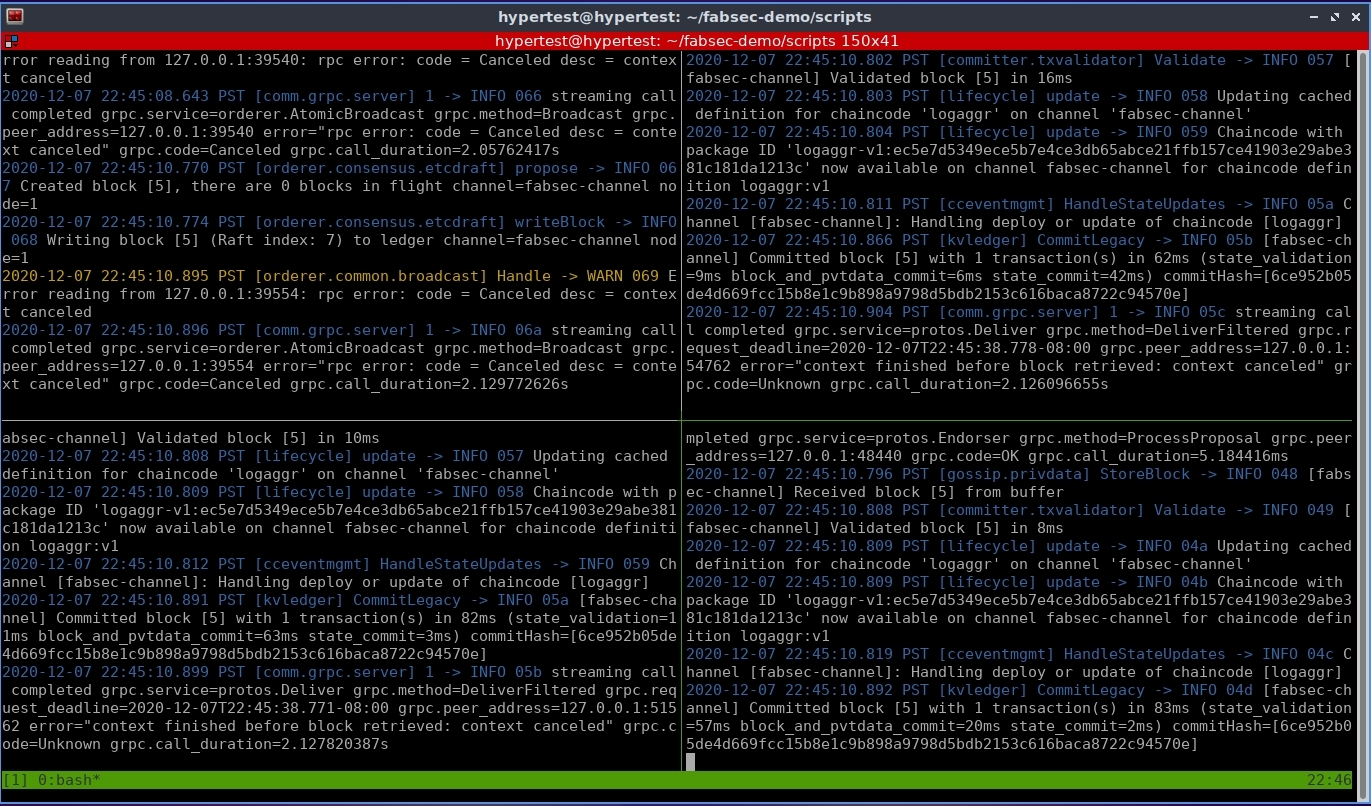
\includegraphics[width=.9\textwidth]{./fabsec-report-network-flow/network-flow-14.jpg}
		\centering
		\caption{Output of Peers After Chaincode Commitment}
		\end{figure}
		
	\newpage
	\hspace{10mm}With the Chaincode deployed and ready to go, we can move to the Frontend/Backend portion of the Javascript code. First we will start with the Backend. The first screenshot show the file layout of each of the main three source directories (for completeness). The second screenshot will show the output of the Backend Javascript modules \textit{enroll-admin.js} and \textit{register-enroll-user.js} for both Organizations.  The third screenshot shows the \textit{watch-and-commit-logs.js} having done their overhead work, and watching for changes to the logfiles. A note here: if you notice that both logfiles are in different place on the filesystem. This is to show one belongs to Organization 1 and one belongs to Organization 2. The fourth screenshot shows these log files populated with unique values, and that those changes were picked up be the Javascript for for both Organizations. Finally, the fifth screenshot shows how the different actors have reacted to the Chaincode being invoked.
	
		\begin{figure}[H]
		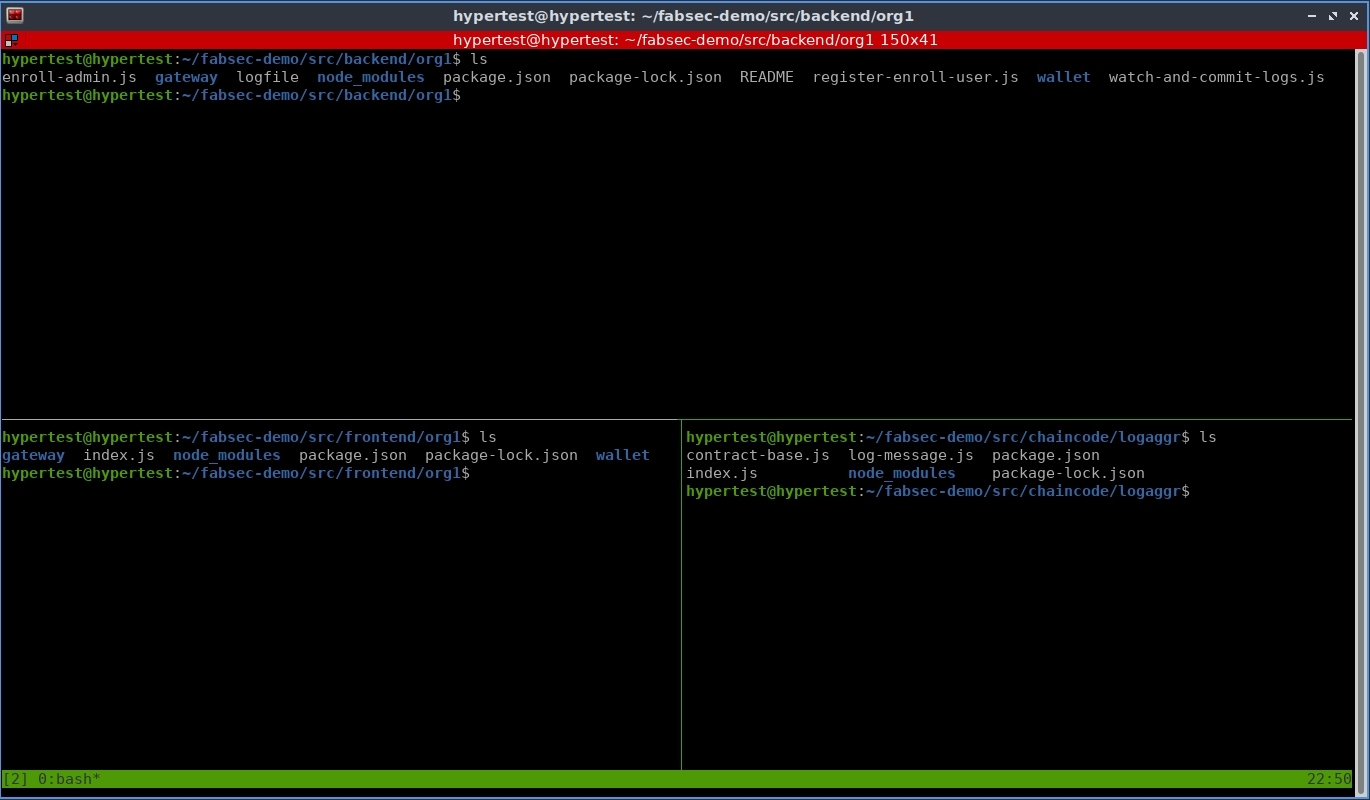
\includegraphics[width=\textwidth]{./fabsec-report-network-flow/network-flow-15.jpg}
		\caption{Directory Listings of the Frontend, Backend, and Chaincode Directories}
		\end{figure}

		\begin{figure}[H]
		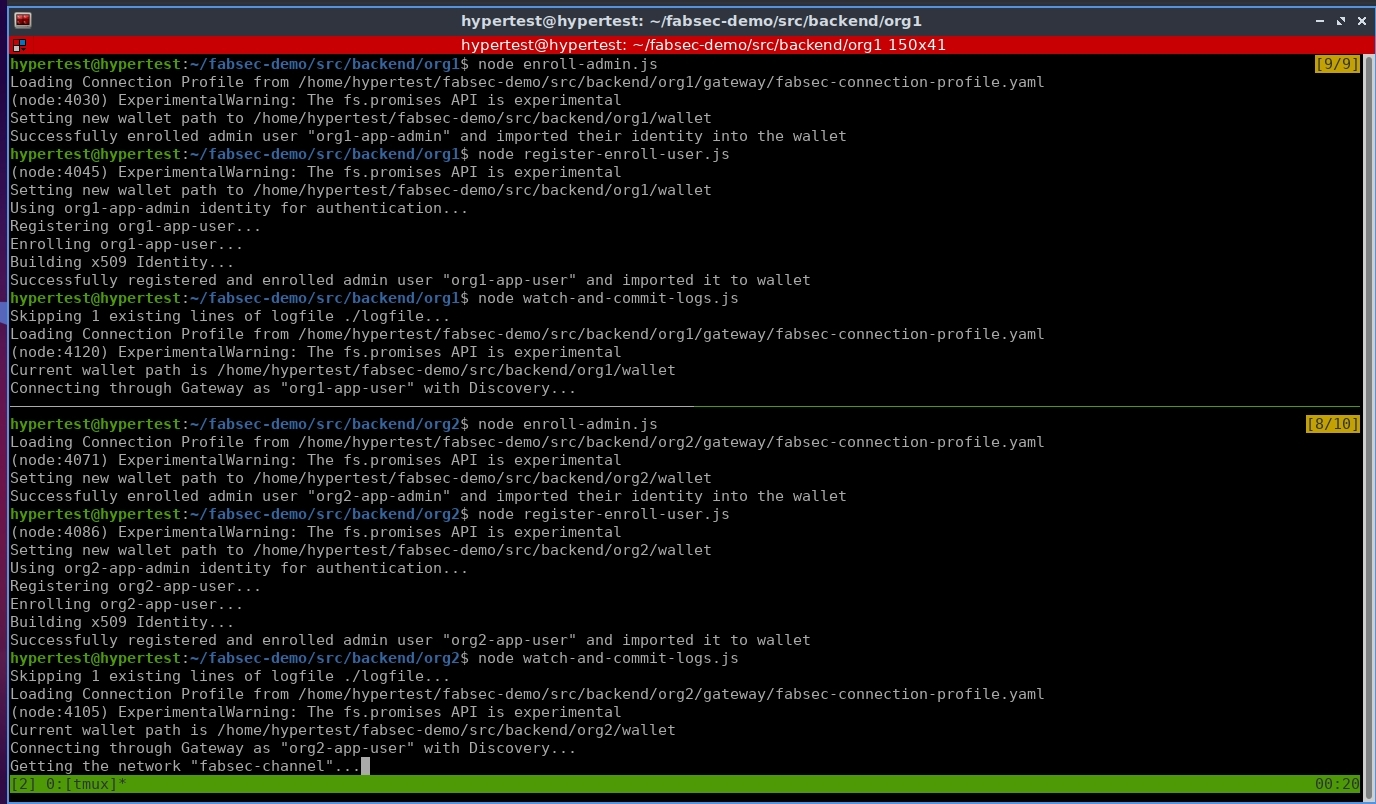
\includegraphics[width=.9\textwidth]{./fabsec-report-network-flow/network-flow-16.jpg}
		\centering
		\caption{Output of the Admin and User Identity Creation}
		\end{figure}
		
		\begin{figure}[H]
		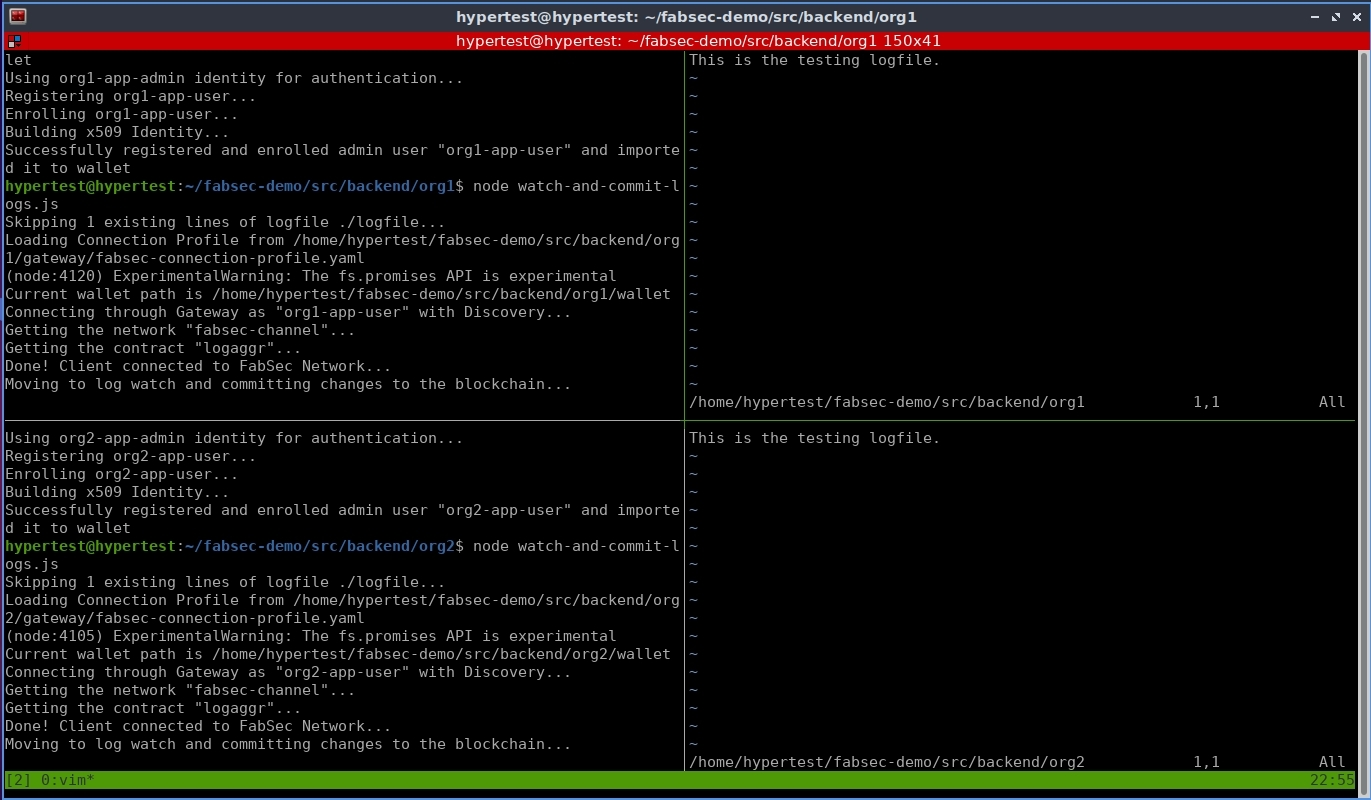
\includegraphics[width=.9\textwidth]{./fabsec-report-network-flow/network-flow-17.jpg}
		\centering
		\caption{Before Log Files Entries Have Been Applied}
		\end{figure}
		
		\begin{figure}[H]
		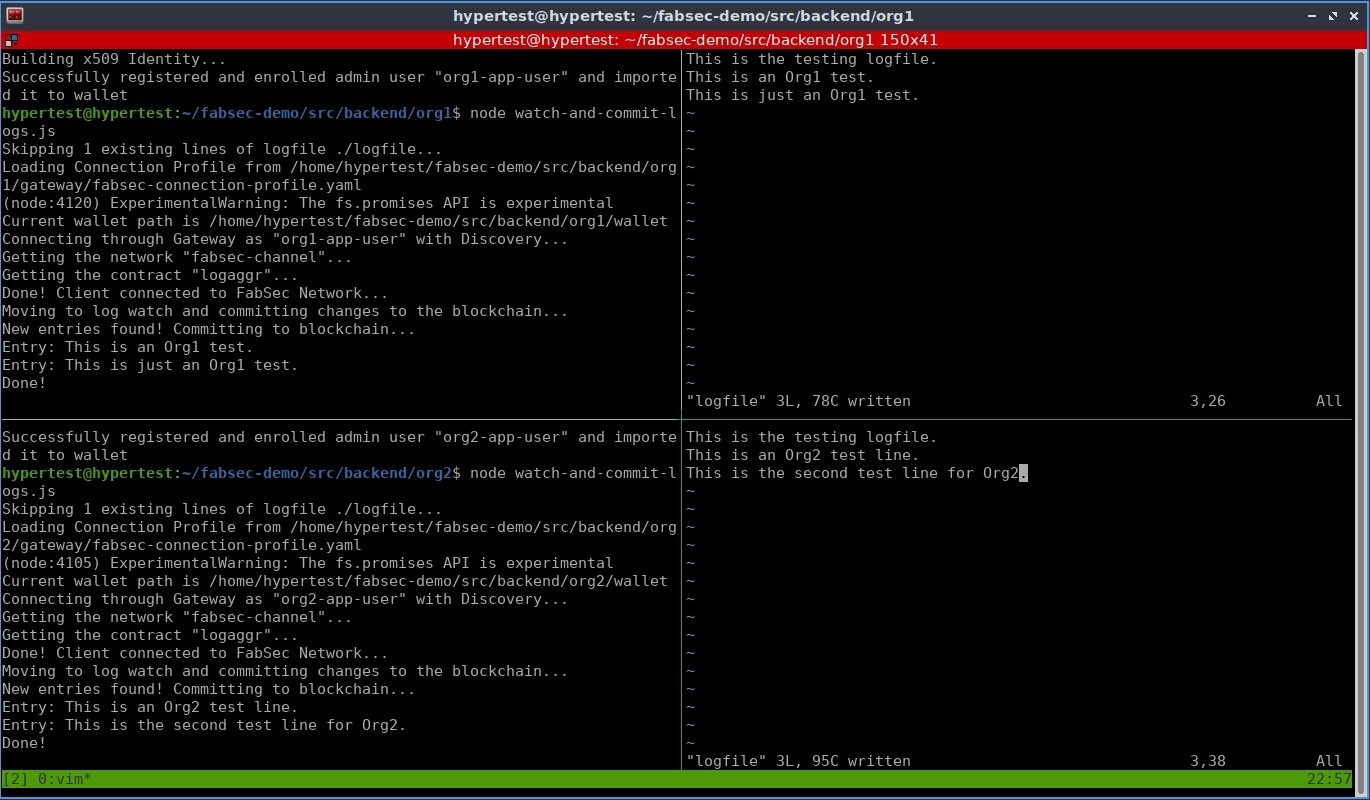
\includegraphics[width=.9\textwidth]{./fabsec-report-network-flow/network-flow-18.jpg}
		\centering
		\caption{After Log Files Entries Have Been Applied}
		\end{figure}	
		
		\begin{figure}[H]
		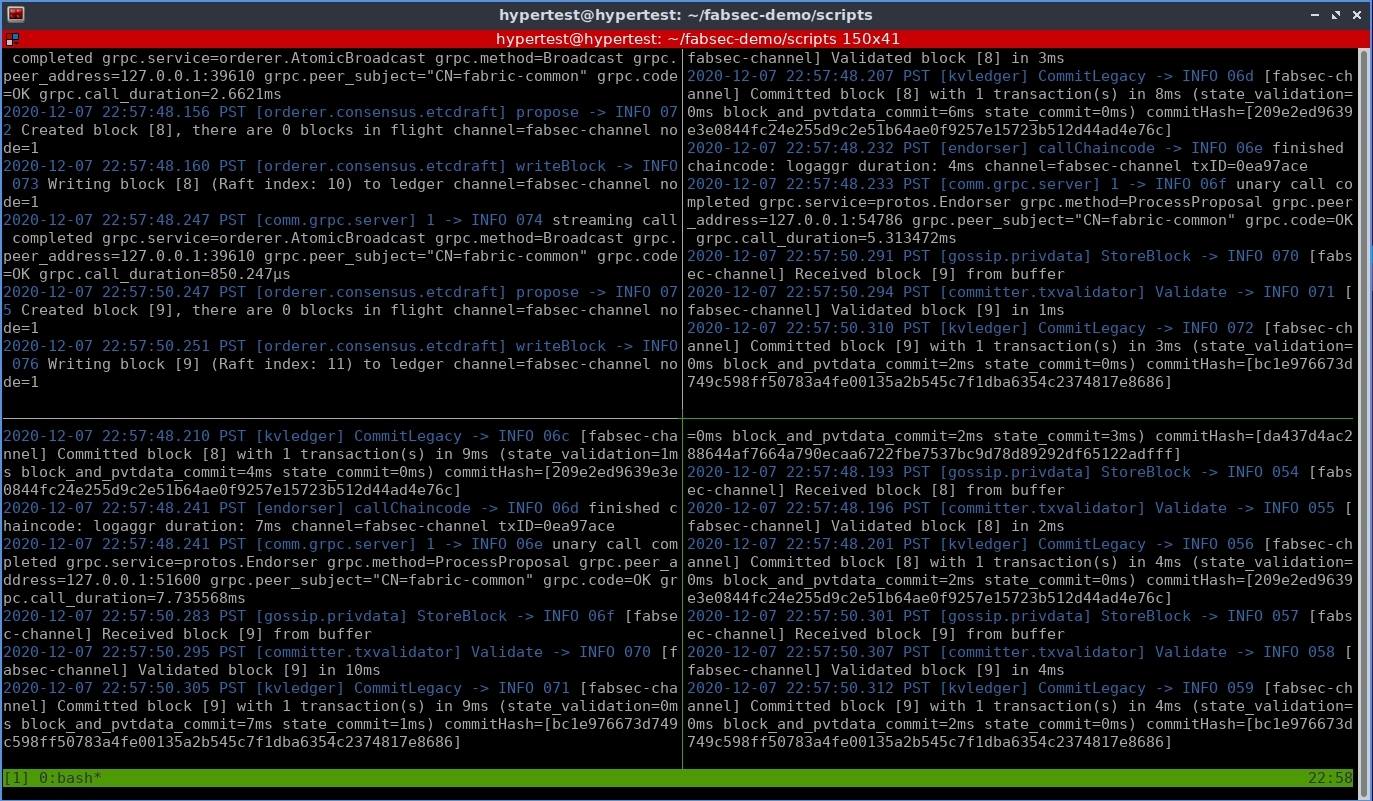
\includegraphics[width=.9\textwidth]{./fabsec-report-network-flow/network-flow-19.jpg}
		\centering
		\caption{Different Reactions of the Chaincode Being Invoked}
		\end{figure}
		
	\newpage
	\hspace{10mm}These last three screenshots show the Frontend in action. The first screenshot shows the Frontend Javascript code being run for both the Organizations. This is done locally, but of course the could be hosted on their individual intranets or even the internet... for some reason. Notice that are running of different ports: 80801 for Org1 and 8082 for Org2. This is to show that they are, indeed, two different entities. The last two screenshots will so a user from Organization 1 accessing the logs, and a user from Organization 2 accessing the logs. Since it's a log aggregator both Organization's users will have the same view.
	
		\begin{figure}[H]
		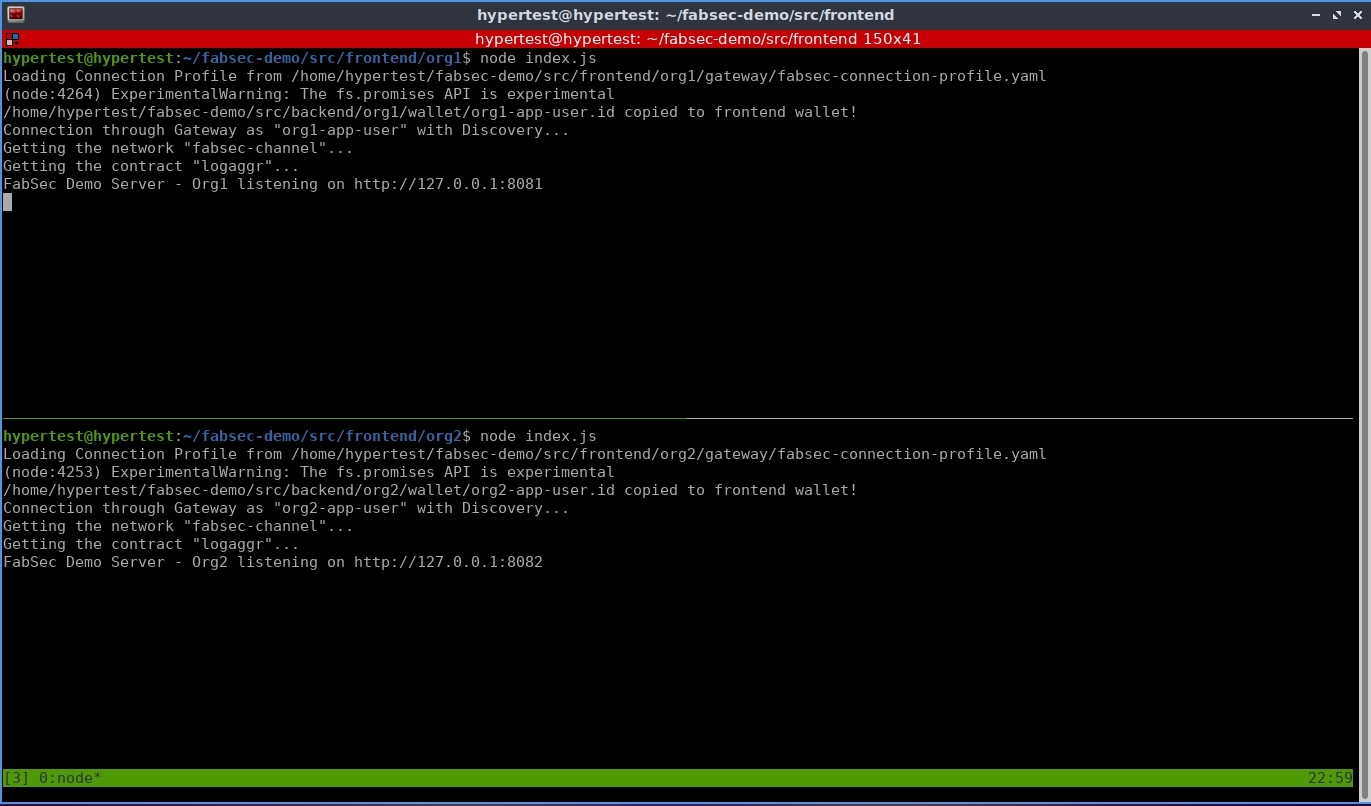
\includegraphics[width=\textwidth]{./fabsec-report-network-flow/network-flow-20.jpg}
		\caption{Output for Frontend Javascript}
		\end{figure}	
		
			\begin{figure}[H]
		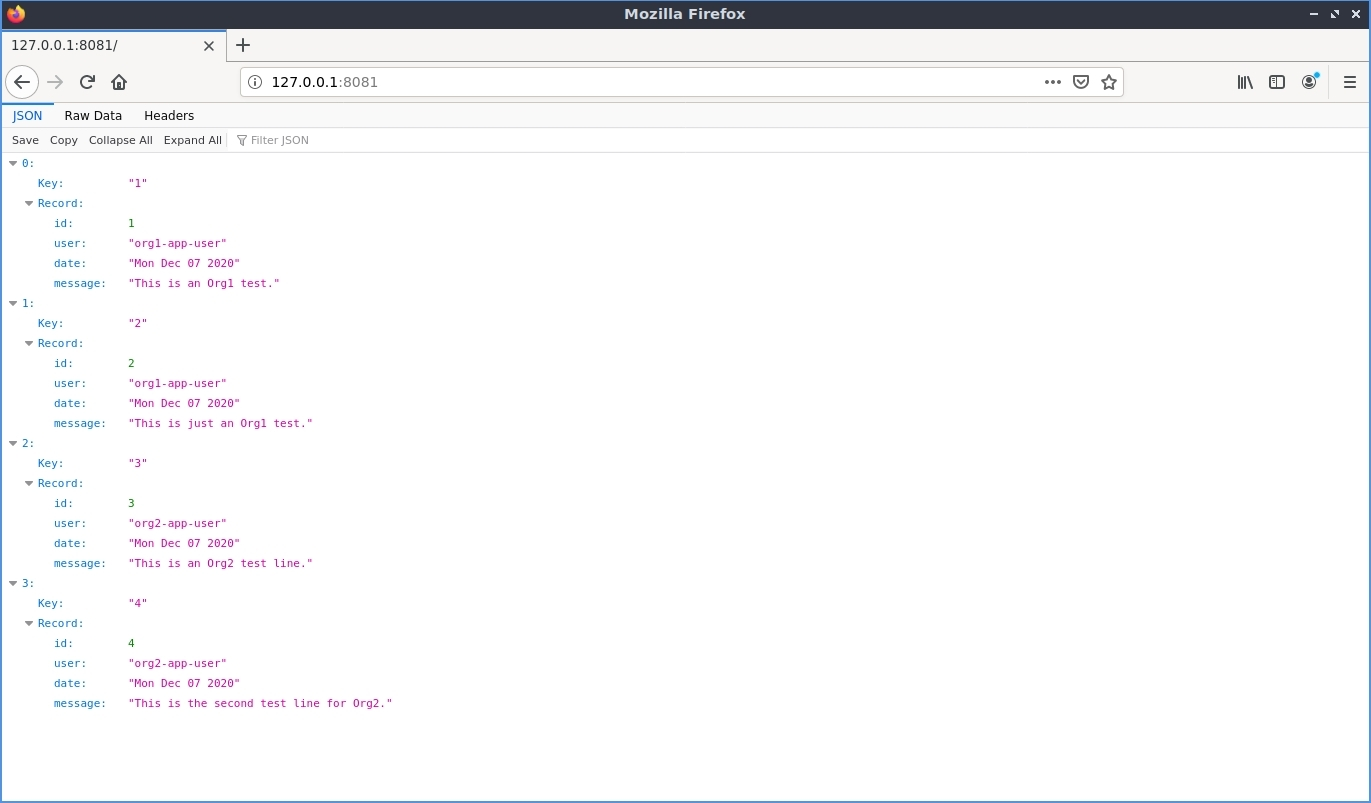
\includegraphics[width=.9\textwidth]{./fabsec-report-network-flow/network-flow-21.jpg}
		\caption{A User at Organization 1's View}
		\end{figure}	
		
		\begin{figure}[H]
		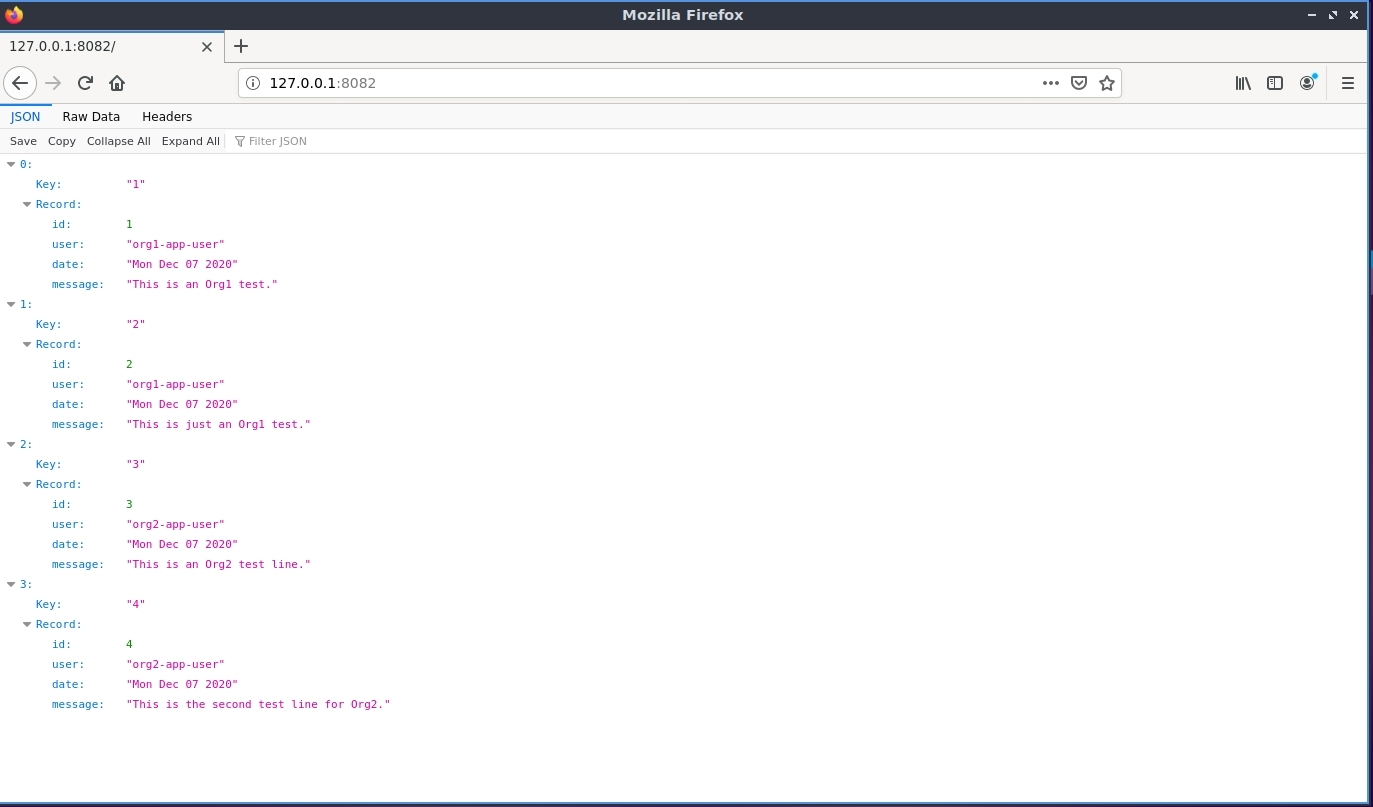
\includegraphics[width=.9\textwidth]{./fabsec-report-network-flow/network-flow-22.jpg}
		\caption{A User at Organization 2's View}
		\end{figure}	
		